\documentclass[conference]{IEEEtran}
\IEEEoverridecommandlockouts
% The preceding line is only needed to identify funding in the first footnote. If that is unneeded, please comment it out.
\usepackage{cite}
\usepackage{amsmath,amssymb,amsfonts}
\usepackage{algorithmic}
\usepackage{graphicx}
\usepackage{textcomp}
\usepackage{xcolor}
\usepackage{hyperref}
\usepackage{textcomp}
\def\BibTeX{{\rm B\kern-.05em{\sc i\kern-.025em b}\kern-.08em
    T\kern-.1667em\lower.7ex\hbox{E}\kern-.125emX}}

% Increase height of cells in tables a bit
\renewcommand{\arraystretch}{1.2}

\begin{document}

\title{Synthesizing Knowledge From Software Development Artifacts: a review}

\author{\IEEEauthorblockN{Christian Paling}
\IEEEauthorblockA{\textit{University of Applied Sciences Regensburg} \\
Regensburg, Germany \\
christian.paling@googlemail.com}}

\maketitle

\begin{abstract}
During the course of a software project, vast amounts of data are being created and stored in software development tools. In case a development team notices that their own development process could be improved, it can be very hard to make sense of the development artifacts which accumulated themselves in their tools. Baysal et al. introduced a pattern called \textit{lifecycle model} to analyse software processes using the data which is stored in software development tools. This review summarises their methodology, the application of the lifecycle model on the code review processes of three projects, and possible findings of such an analysis.
\end{abstract}

\begin{IEEEkeywords}
Software Processes, Code Review, Lifecycle Model
\end{IEEEkeywords}

\section{Introduction}

Code review has established itself as a very popular technique in the software industry. Empirical studies have shown that incorporating code review into software projects improves not only the design of a software system but lowers the defect proneness of software as well \cite{mcintosh2016empirical}\cite{morales2015code}.

According to the authors of the underlying work of this review (see \cite{baysal2015synthesizing}), code review is especially important for open source software development. While open source projects generally have core developers who handle most of the work of the project, bug fixes, features, or documentation often come from a larger community as well. Core developers, therefore, have to act as gatekeepers and have to decide which patches are merged into the code base, and which are rejected. Because of the significance of code review for open source projects, it is important to analyse one's own code review process to spot problems or rooms for improvement.

However, not only the data of the code review process is being created during the course of a project. Issue tracking software or version control systems contain vast and various amounts of development artifacts that are ready to be analysed to gain insights about the processes of software development teams and projects. Since it can be easy to get lost in the data which accrued itself over time, the question arises how to analyse these quantities of data, and how to spot these above-mentioned rooms for improvement.

Olga Baysal, Oleksii Kononenko, Reid Holmes, and Michael W. Godfrey have presented a methodology to tackle a problem like this, by using the example of code review. In their work, the authors analysed the code review processes of the Mozilla, WebKit, and Blink project. While Mozilla is well-known and requires no additional introduction, WebKit and Blink should be explained in further detail (taken from~\cite{baysal2015synthesizing}): WebKit is an HTML layout engine to render web pages and execute JavaScript code. Multiple companies contributed to the WebKit project, including Google, Apple, and BlackBerry. In 2013, Google forked WebKit and introduced the Blink project because they wanted to perform deeper changes. 

To perform this analysis, the authors presented and utilized \textit{artifact lifecycle models} and combined them with their available data. With their models, the researchers tried to find out whether patches are equally treated in the Mozilla project, i.e. regardless of whether the contributor is a \textbf{core} or \textbf{casual} developer regarding his experience of the Mozilla project. Furthermore, they tried to compare the code review processes across the Mozilla, WebKit, and Blink project. The results show the practicality of their methodology, and that lifecycle models are able to provide interesting insights, like the positive impact of an automatic test system on code review, or how it's more likely to receive a response as a core developer compared to a casual developer.

This review summarises the methodology, its application to real-life code review processes, and the insights of Olga Baysal et al. The review concludes with a deeper look at related work on the topic of code review. The original work appeared in \textit{The Art and Science of Analyzing Software Data} published by \textit{Elsevier} with the title \textit{Synthesizing Knowledge From Software Development Artifacts}.

\section{Methodology}

\subsection{Lifecycle Model}

To organise the amount of information on code review which is stored in development tools like Bugzilla, the authors introduced a pattern called \textit{lifecycle model}, which is described in further detail as follows \cite{baysal2015synthesizing}: the lifecycle model is basically a graph of the possible states through which a certain type of data can flow and change over the course of time. The model is therefore applicable to data that changes its state over time. Issues in issue tracking systems are a good example: they could possibly start with a state of \textit{OPEN} and could end with either \textit{RESOLVED} or \textit{WONTFIX}. A possible insight that the lifecycle model could highlight in this case, would be the number of bugs that were opened from the state \textit{WONTFIX}.

\pagebreak

To generate a lifecycle model, the authors define the following three steps \cite{baysal2015synthesizing}:

\begin{enumerate}
    \item Define the states of the system or process.
    \item Define the possible transitions between each state.
    \item Define the finite states.
\end{enumerate}

After the creation of the model by using these three steps, it can be applied and combined with the available data to get quantitative results for each state and transition. Furthermore, an additional possibility of the model is the tracking of time that is spent until a certain transition occurs.

In Figure \ref{fig:example_model}, the authors generated the lifecycle model for the code review process of the Mozilla project. The subsequent explanation illustrates how to read and understand such a model~(see \cite{baysal2015synthesizing}): the process begins with a request for either a review or a super-review (labeled as r? and sr? respectively). The former type of review can be performed by anyone with knowledge of the module which is being changed, while the latter can only be reviewed by a few selected core developers of Mozilla. Super-reviews are requested when a patch modifies vital core functionality. After the request for a review, the patch enters the \textit{Submitted} state. From here, the patch can reach the terminal state \textit{Timeout} in case it never receives an answer, or it can enter the \textit{Accepted} or \textit{Rejected} state after being marked with \textbf{+} or \textbf{--} by a reviewer. Accepted patches as well as rejected patches can be accepted or rejected multiple times. Furthermore, an accepted patch can be rejected at a later point in time and vice versa. Lastly, the four terminal states are defined as follows:

\begin{itemize}
    \item \textit{Landed}: patches that were incorporated into the codebase.
    \item \textit{Resubmitted}: patches that were submitted again after receiving an answer.
    \item \textit{Abandoned}: patches that were not improved after being rejected.
    \item \textit{Timeout}: patches that never received an answer.
\end{itemize}

\begin{figure}
    \centering
    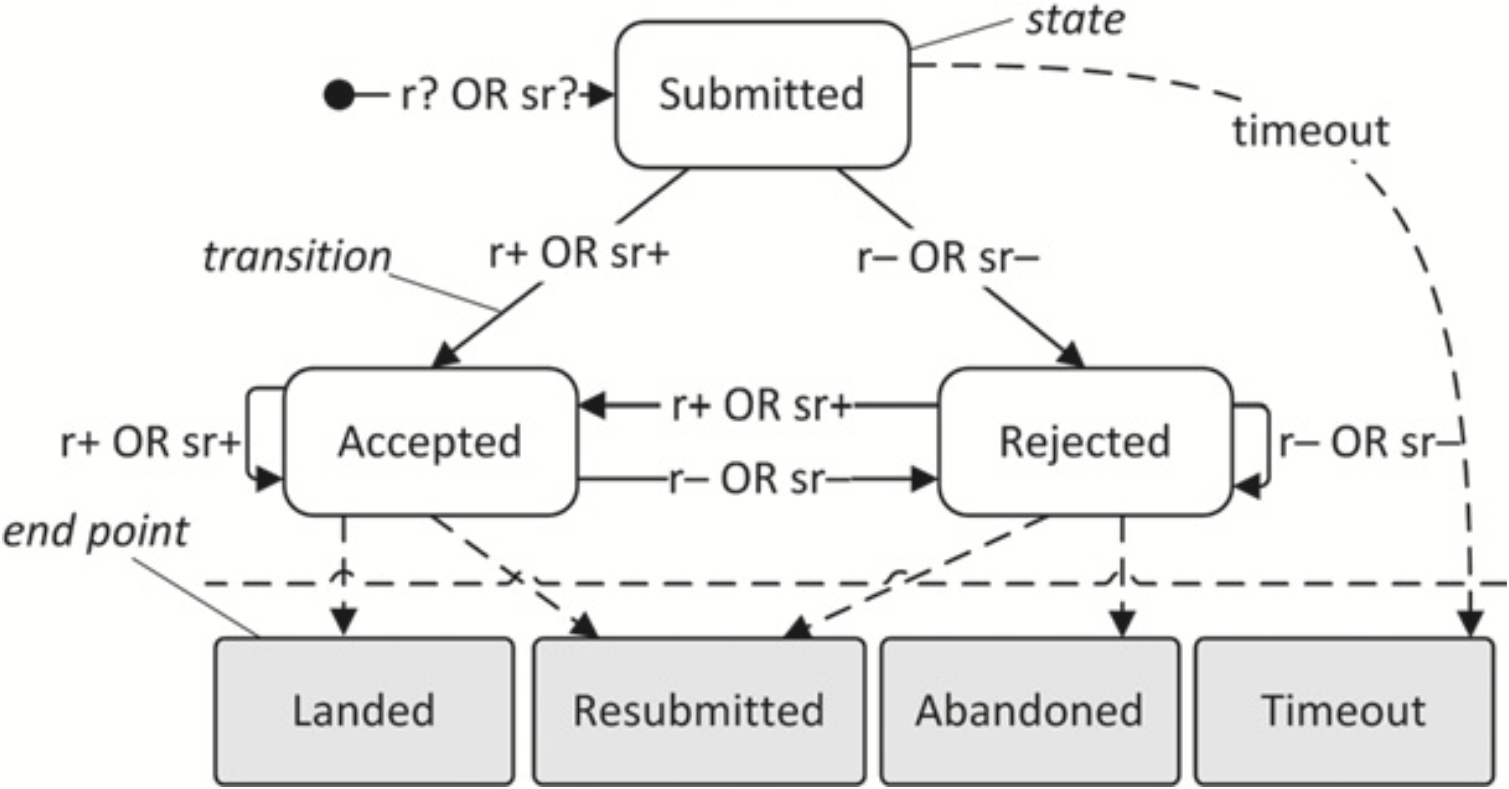
\includegraphics[scale=0.15]{img/example_lifecycle_model.png}
    \caption{Patch lifecycle for the Mozilla project\cite{baysal2015synthesizing}.}
    \label{fig:example_model}
\end{figure}

Finally, it is important to remark, that the sum of all patches in the four terminal states must be equal to the number of patches that were initially submitted \cite{baysal2015synthesizing}.

Because Mozilla does not employ super-reviews anymore~\cite{mozilla_super_review}, the lifecycle model would look slightly different at the time of writing.

\subsection{Data Extraction}

Although Baysal et al. do not explicitly describe their process of extracting the data they used for their analysis in the reviewed work, in other papers of the same authors where lifecycle models were utilized, their process of retrieving the underlying data is more clearly outlined (see \cite{baysal2013influence}):

First, the authors scraped all data from the project's issue repository, in this case, Bugzilla, which was submitted during a fixed time span. For all patches, the metadata was extracted, including the submission date, the person who submitted the patch, number of lines added and removed, and all details concerning the review of the patch. After having downloaded all the raw data, the researchers removed all outliers from the data set. For example, patches which took much longer to receive an answer than the median review time were removed. In the end, the authors had a large data set available that was ready to be applied and analysed using a generated lifecycle~model.

To reproduce the results which are presented next, the following time spans and thresholds were used to extract and categorize the data. For the Mozilla project, the approach of the researchers is described in the following way (see \cite{baysal2012secret}): the patches, which were utilized for the lifecycle models in the reviewed work, were all submitted between April 12, 2011, and April 12, 2012. Furthermore, to decide whether a contributor belongs to the core or casual group, the researchers analysed all patches which were submitted during a two-year timespan (which was not specified in detail), and chose to set the casual group to 20 or fewer patches, and the core developer group to 100 or more patches. Patches from developers between 20 and 100 were left out of the analysis.

For the WebKit model, the authors did not categorize their data, however, all patches were submitted between April 12, 2011, and December 12, 2012\cite{baysal2013influence}.

Lastly, details concerning the data extraction for the Blink project were not presented in the reviewed work or in referenced works.

\section{Detailed Results}

\subsection{Mozilla Project}

In Figure~\ref{fig:mozilla_core_dev}, the authors have applied all the patches of the core developers of the Mozilla project on their lifecycle model. Since Figure~\ref{fig:example_model} was already a lifecycle model of the code review process of Mozilla, there is no change concerning the states and possible transitions. The only difference is that each transition now has some quantitive information annotated to it.

During the time span of the analysis, 1,419 patches were submitted by core developers. From each state, the amount of patches that changed to a next state is specified as a percentage, e.g. from the \textit{Submitted} state, 82\% of the reviews were accepted, 17\% were rejected and 0.6\% did not receive an answer.

\pagebreak

\begin{figure}
    \centering
    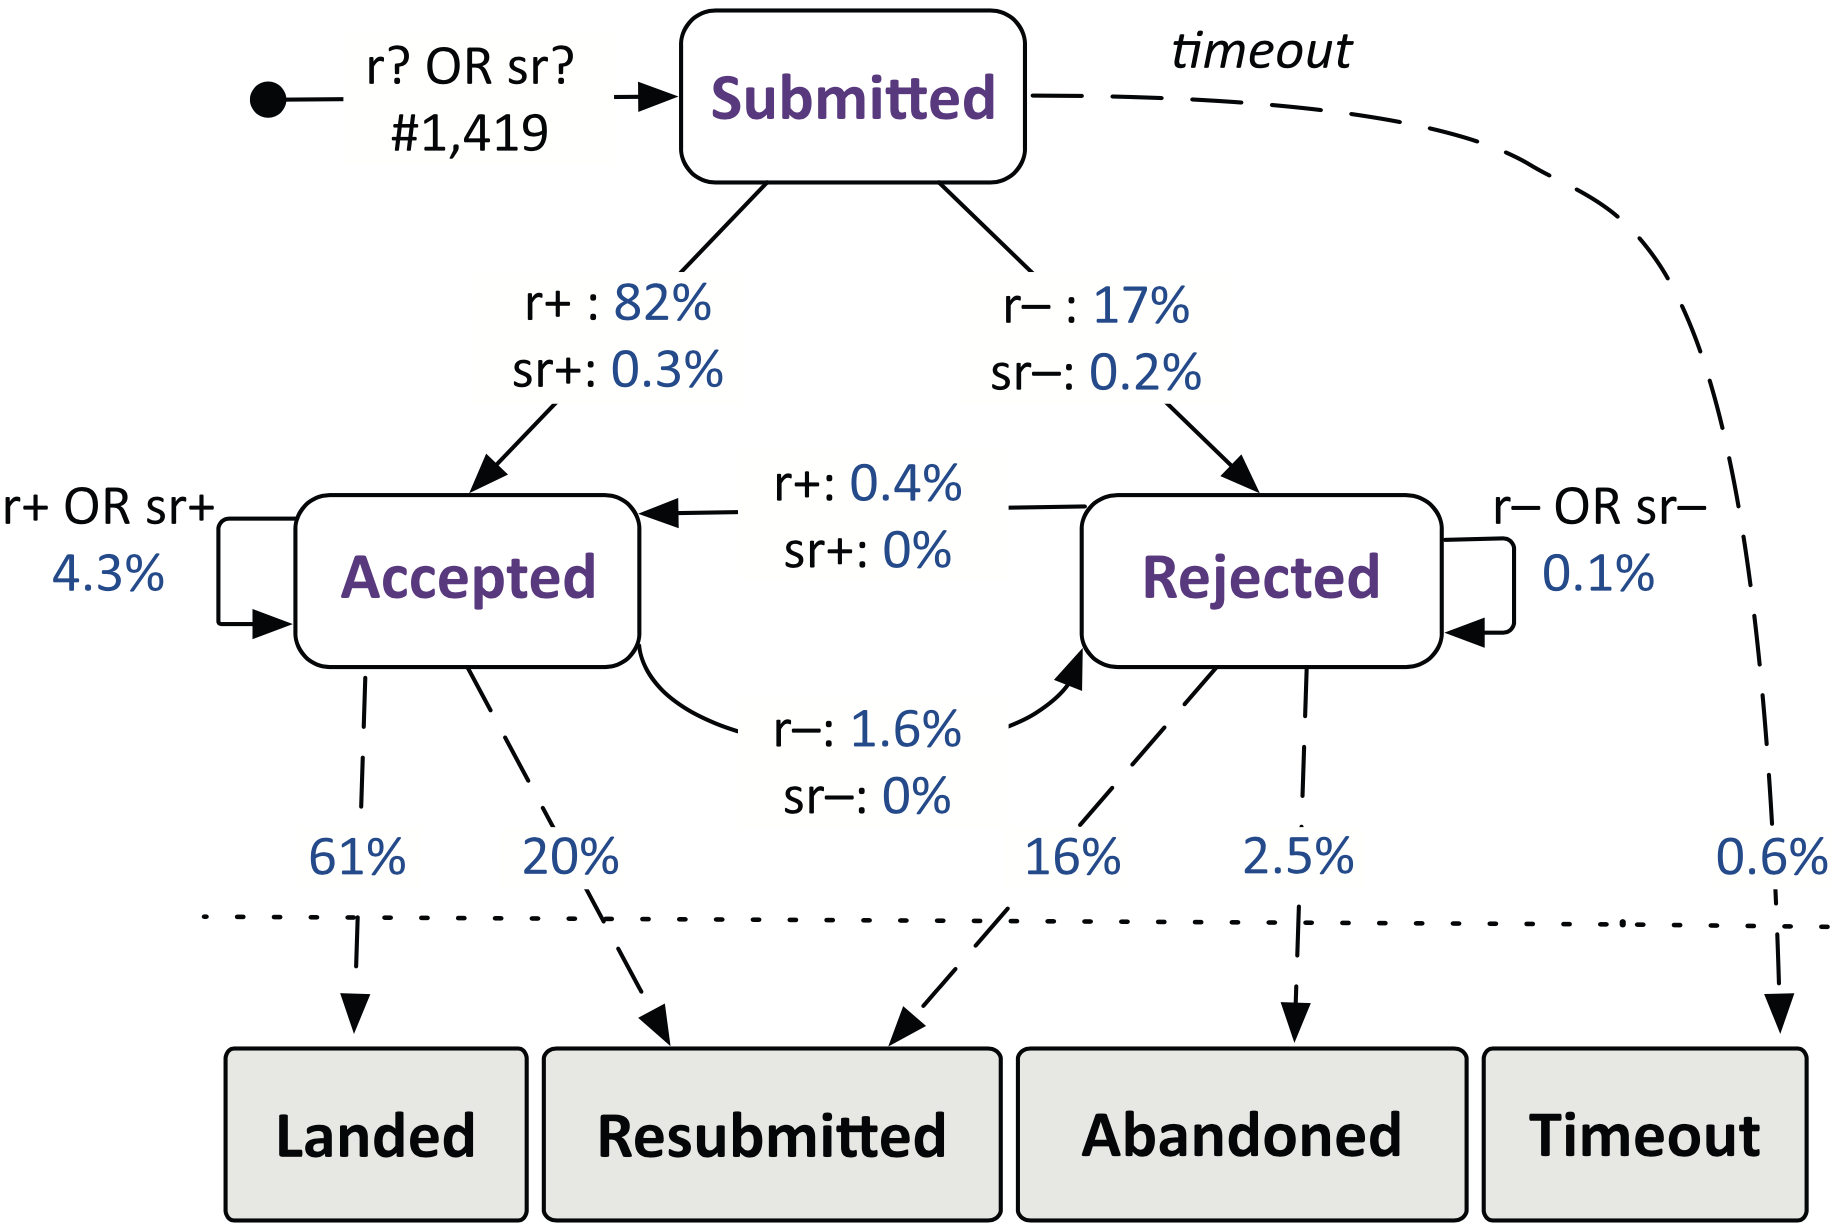
\includegraphics[scale=0.23]{img/mozilla_core_developers.png}
    \caption{Mozilla's patch lifecycle for core developers \cite{baysal2015synthesizing}.}
    \label{fig:mozilla_core_dev}
\end{figure}

When comparing these results to the patch lifecycle for casual developers in Figure~\ref{fig:mozilla_casual_dev}, the following differences are apparent: the amount of positive reviews is 7\% lower than for the core developers, and the amount of negative reviews is 6\% higher. The number of patches reaching \textit{Landed} is also lower than for the core developers which indicates that it is less likely to get a patch merged as a casual developer. Furthermore, casual developers receive more than three times as often no answer compared to core developers. Lastly, the amount of reviews landing in the \textit{Abandoned} state is more than three times higher as well.

In Figure~\ref{fig:mozilla_casual_dev}, a small error in the lifecycle model is visible: as stated before, the sum of the patches reaching the terminal states must equal the number of patches that were initially submitted, i.e. they must amount to 100\%. It is likely that the amount of patches that are resubmitted after being rejected, is much lower than the 68.5\% which is given in the lifecycle model of the authors. During the writing of this review, the authors of the reviewed work did not respond to an inquiry for a revised lifecycle model.

\begin{figure}
    \centering
    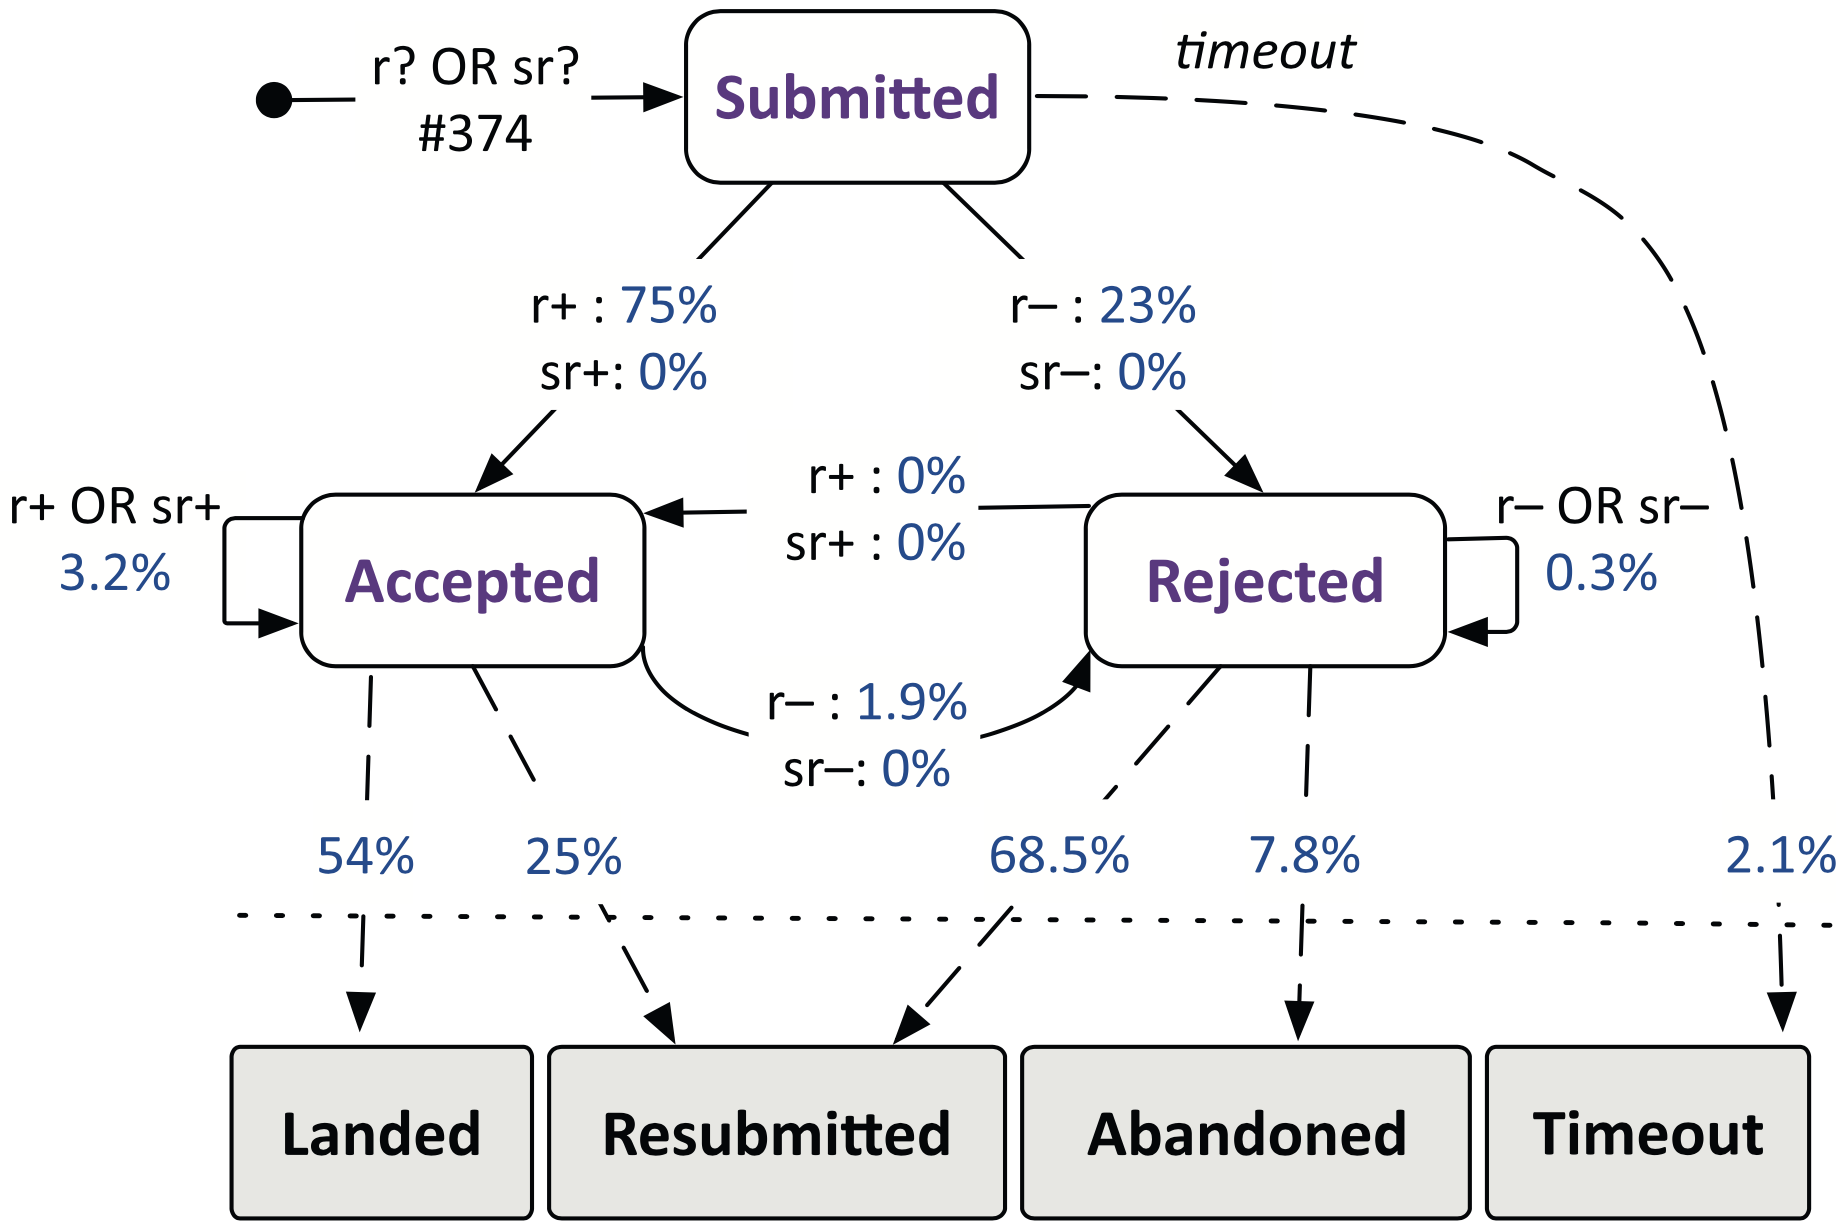
\includegraphics[scale=0.23]{img/mozilla_casual_developers.png}
    \caption{Mozilla's patch lifecycle for casual developers \cite{baysal2015synthesizing}.}
    \label{fig:mozilla_casual_dev}
\end{figure}

However, not only quantitive insights can be gained by analysing processes using lifecycle models. As stated before, it is also possible to track the time it takes until some data transitions to a subsequent state. In Table~\ref{tab:mozilla}, the median time for each transition was tracked and calculated. It is evident that negative responses generally took longer than positive responses, and super reviews took longer than normal reviews. For the casual contributors, no super review was requested, therefore no median time could be acquired. It is important to keep the underlying data in mind during the course of the analysis. In the case of the transition \textit{r--$\,\to\,$r+}, the median time for casual contributors is very low compared to the time of core contributors because there is only one patch that transitioned from \textit{Rejected} to \textit{Accepted} for the casual developers \cite{baysal2015synthesizing}. The result, in this case, is therefore not representative and could generate misleading insights.

\begin{table}[htbp]
\caption{Median Time of Transition (Minutes) for Mozilla Firefox\cite{baysal2015synthesizing}.}
\begin{center}
\begin{tabular}{|c|r|r|}
\hline
\textbf{Transition} & \textbf{Core Contributors} & \textbf{Casual Contributors} \\
\hline
r?$\,\to\,$r+ & 534 & 494 \\
\hline
r?$\,\to\,$r-- & 710 & 1024 \\
\hline
r+$\,\to\,$r-- & 390 & 402 \\
\hline
r--$\,\to\,$r+ & 1218 & 15 \\
\hline
sr?$\,\to\,$sr+ & 617 & n/a \\
\hline
sr?$\,\to\,$sr-- & 9148 & n/a \\
\hline
\end{tabular}
\label{tab:mozilla}
\end{center}
\end{table}

\subsection{WebKit Project}

The lifecycle of the WebKit project in Figure~\ref{fig:webkit} reveals interesting differences compared to the process of Mozilla. First of all, there are new transitions, e.g. it is possible to resubmit a patch immediately after it was submitted, and it is not possible to accept or reject a patch multiple times. But not only does the process of WebKit contain new transitions between states, the transition between \textit{Submitted} and \textit{Resubmitted} amounts to about one third of all patches. This implies that there are some differences between the code review process of Mozilla and WebKit. The researchers found out, that the cause for having this new transition between \textit{Submitted} and \textit{Resubmitted} can be attributed to the automatic test system of WebKit, which helps developers to know immediately after submitting whether their patch contains a mistake or not\cite{baysal2015synthesizing}.

\begin{figure}
    \centering
    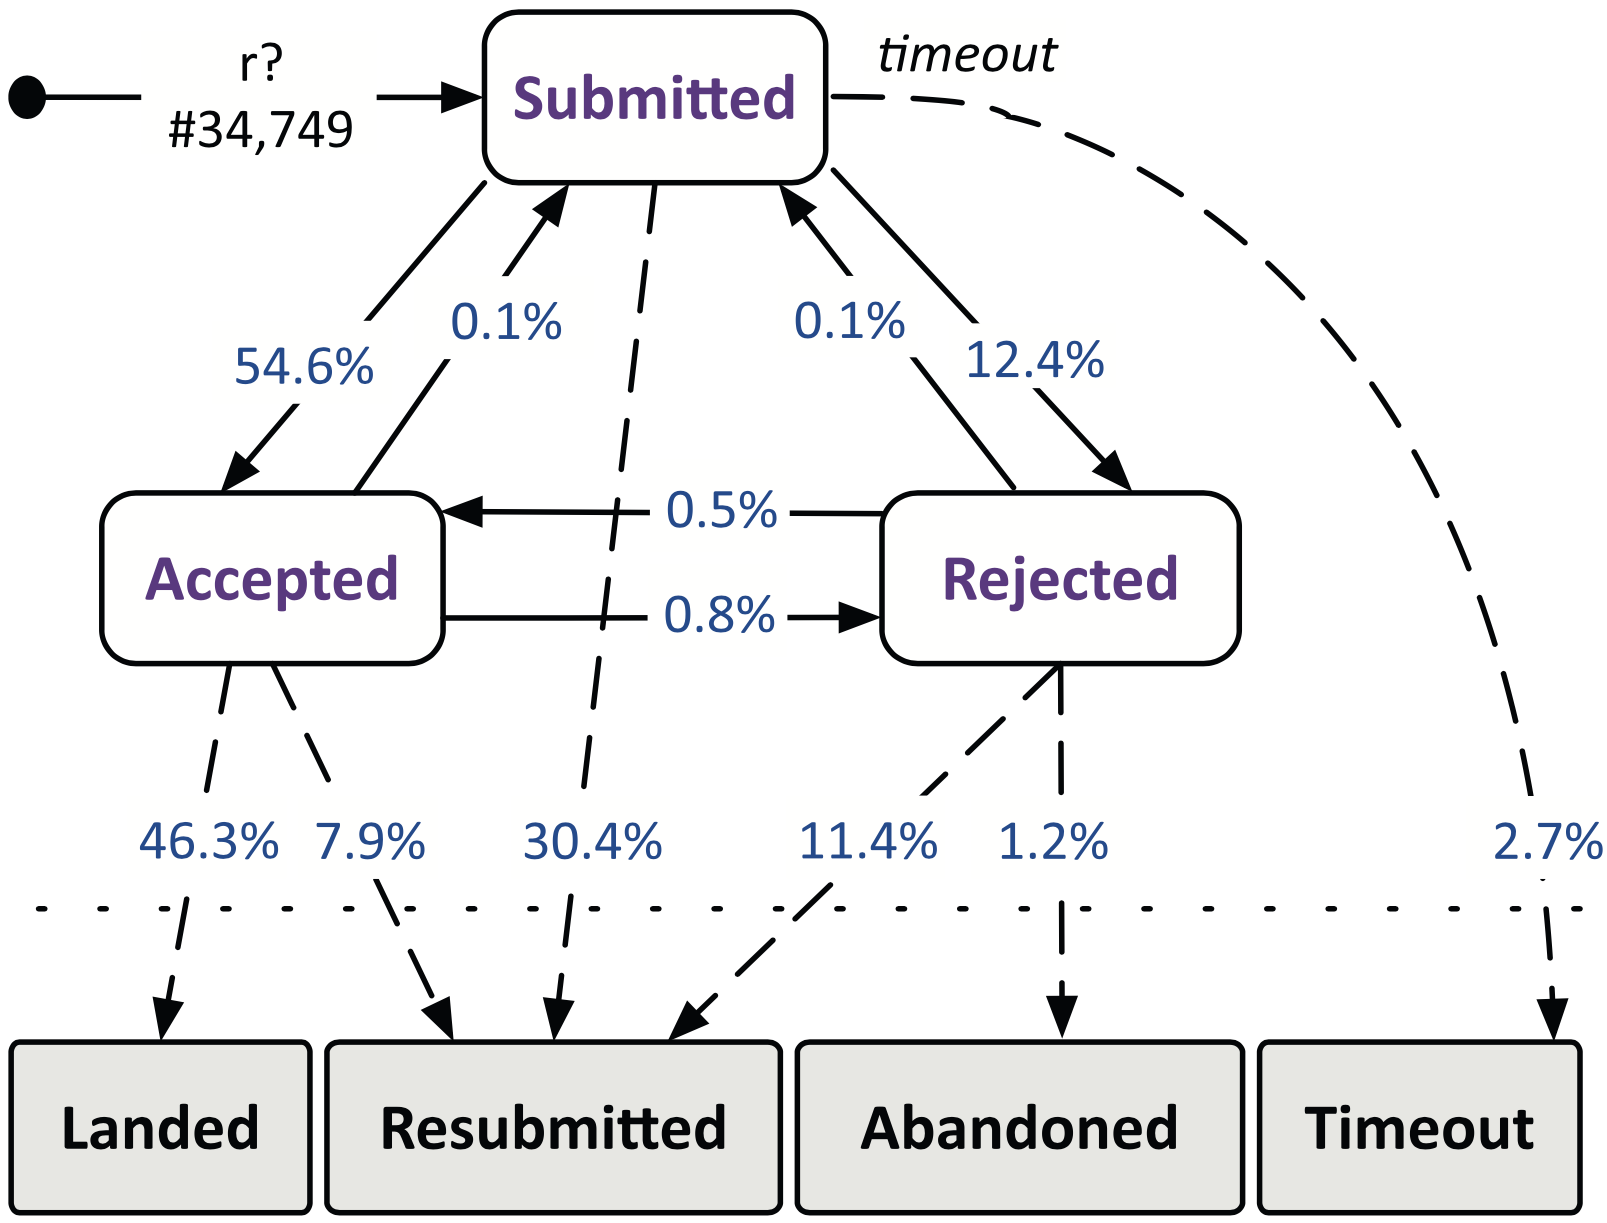
\includegraphics[scale=0.25]{img/webkit.png}
    \caption{WebKit's patch lifecycle \cite{baysal2015synthesizing}.}
    \label{fig:webkit}
\end{figure}

\subsection{Blink Project}

Lastly, the code review process of the Blink project in Figure~\ref{fig:blink} is generally similar to the one of WebKit. There are a few differences, nonetheless. First of all, in the Blink project, it is allowed to merge changes directly into the code base without any review. According to the authors, the developers do this for small changes or bug fixes which were not included in the actual patch \cite{baysal2015synthesizing}. Furthermore, the amount of patches receiving a negative answer is quite low compared to Mozilla and WebKit. According to Baysal et~al.\cite{baysal2015synthesizing}, this is the result of the reviewing mindset of the Blink project, where the reviewers do not want to give a patch a negative response which could possibly discourage the author to participate further and improve his submission. The developers of Blink, therefore, try to discuss improvements in the \textit{Submitted} state until they are able to accept the patch. However, this mindset results in a higher amount of patches that do not receive any review response because instead of abandoning the patch in the \textit{Rejected} state, authors abandon the patch in the \textit{Submitted}~state.

\begin{figure}
    \centering
    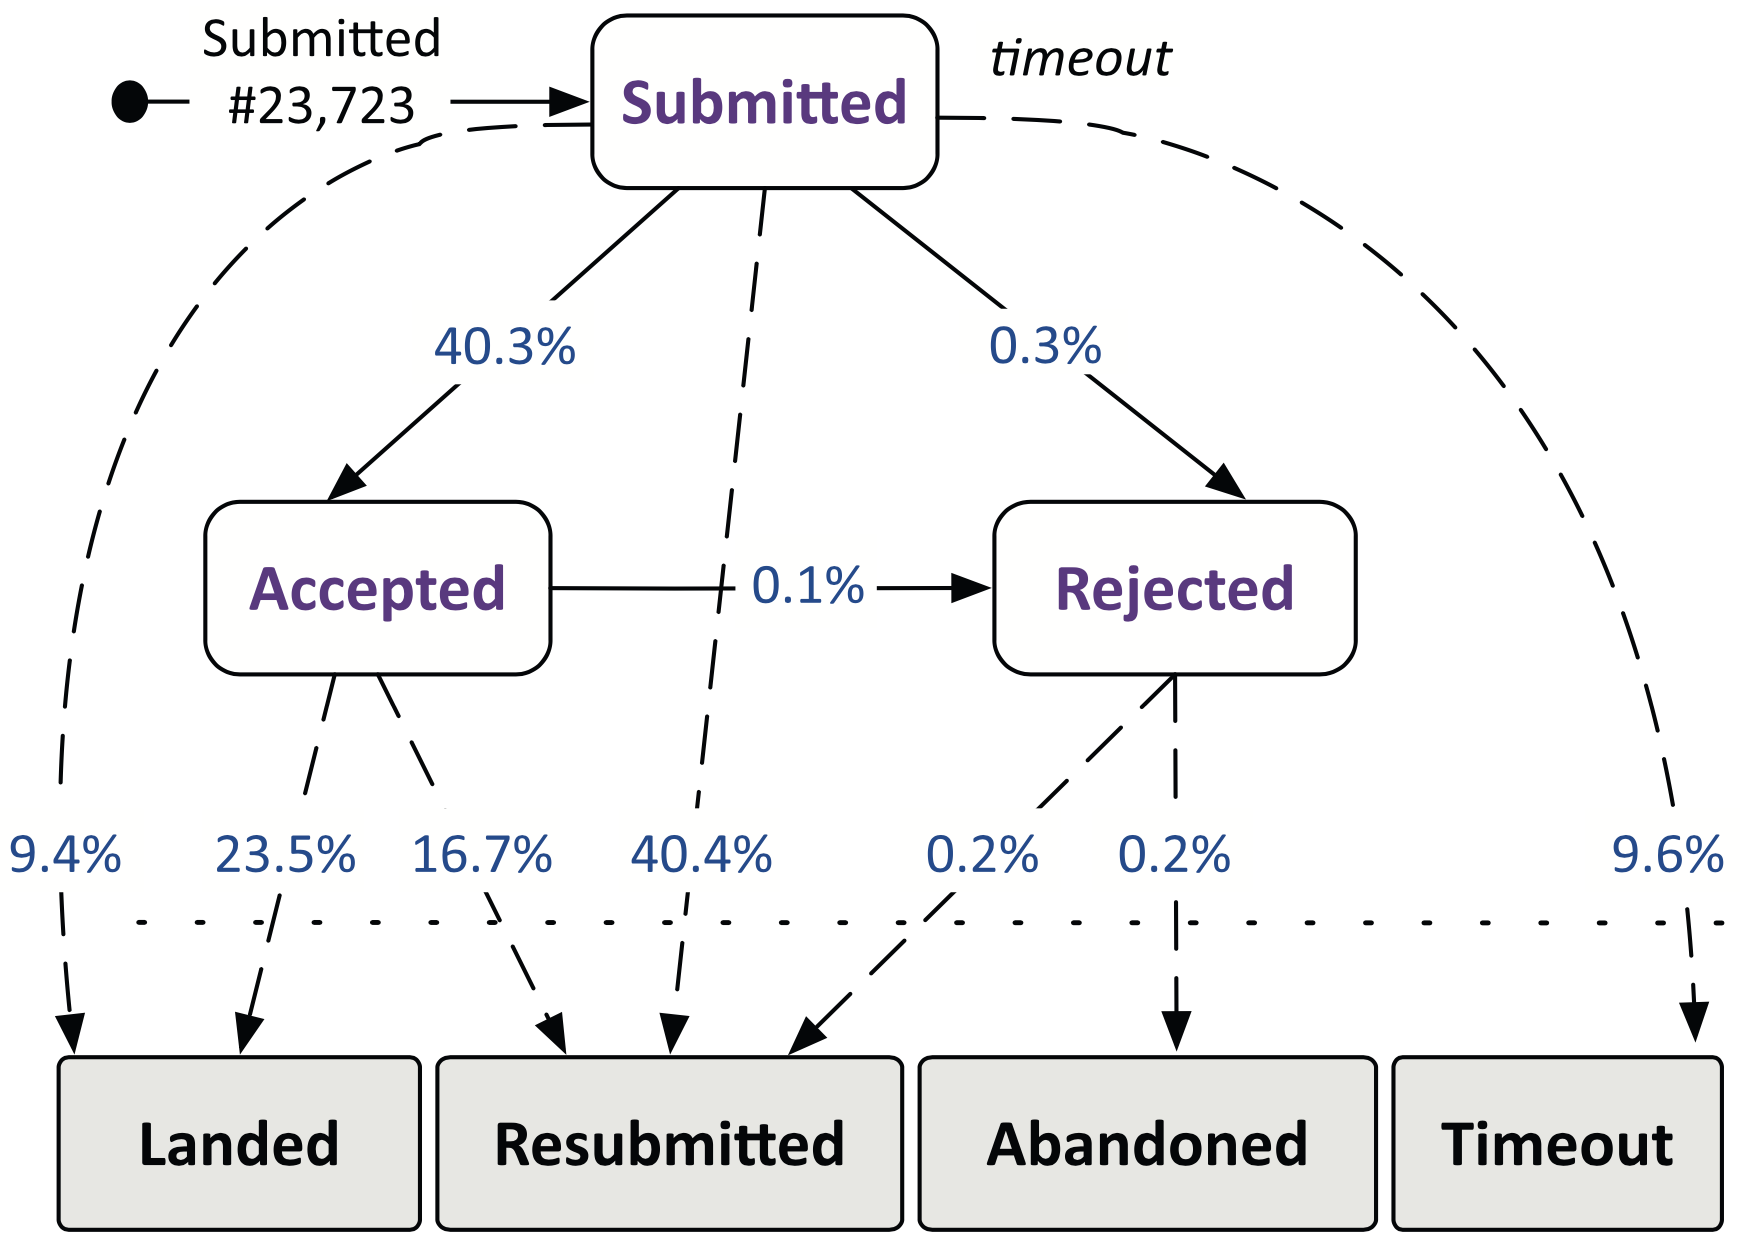
\includegraphics[scale=0.25]{img/blink.png}
    \caption{Blink's patch lifecycle \cite{baysal2015synthesizing}.}
    \label{fig:blink}
\end{figure}

\section{Discussions}

The results of the comparison between the core and casual developers for the Mozilla project showed that patches from casual developers are more often abandoned by either the developer or the reviewer. This generated some discussion and concerns among the developers of the Mozilla team who agreed that "it's worth looking into the "abandoned" data set more carefully to see what happened to those patches" \cite{baysal2015synthesizing}.

The high amount of patches, which are immediately resubmitted due to a failure in the automatic test system in the WebKit and Blink project, is an indication for the effectiveness of continuous integration (CI) for code review. The CI system is able to find defective patches right away without a reviewer having to take a look at the code. This can, first of all, save valuable time for the reviewers of the project, and secondly, help to prevent having bugs in the code base in case a flawed patch is erroneously accepted.

Lastly, with the help of the lifecycle models, it was possible to get an impression of the code review process of the different projects. As an example, Blink is the only project that allows patches to be merged into the code base without any review at all. This indicates, that the code review process of Google for the Blink project may not be as strict as the one of WebKit or Mozilla \cite{baysal2015synthesizing}.

\section{Threats to Validity}

Baysal et al. point out a few threats to validity in their underlying paper which described the analysis of the Mozilla project \cite{baysal2012secret}:

Firstly, the assessment of a code review process using a lifecycle model is heavily related to the project for which the model was created. Although the lifecycle model can be easily adapted to other code review processes, the results can usually not be generalized. The authors also point out that resubmissions in the lifecycle model are determined by analysing whether a certain bug has multiple patches assigned to it. This means that patches on the same bug report are assumed to never be independent of each other. According to the authors, this assumption holds in most of the cases.

The authors seem to additionally validate their data extraction and findings by contacting the organisations of the projects. For the WebKit project, the researchers got in touch with individuals from Apple, Google, and Intel to get more insights into internal processes \cite{baysal2013influence}.

Lastly, an important aspect and a possible source of errors concerning the generation of a lifecycle model is the chosen time frame of the data that should be analysed. In case the time span is too short, the results might not be representative for the overall process. A time span that is too long, however, might yield results that do not show effects of internal, process-related changes that occurred during the time span. The results which the lifecycle model produces could, therefore, be diluted by outdated data. 

\section{Related Work}

There is a multitude of work related to the analysis of code review processes. In the work of Baysal, Kononenko, Holmes, and Godfrey which explored the WebKit project, which also was part of this review, the authors did not only generate a lifecycle model for WebKit's patch lifecycle but also utilized the model to investigate effects of non-technical factors on code review. The results of the work support also the findings that were discussed in this review. The researchers found that the more a developer participates in the project, the faster and more likely his changes will be reviewed and incorporated into the code base \cite{baysal2013influence}.

In 2015, Kononenko et al. again studied the Mozilla project to try to find effects of personal factors on the quality of code review. In their study, they showed that 54\% of all reviewed changes still introduced bugs in the code, and their results suggested that the review experience and current review load can be predictors of code review quality \cite{kononenko2015investigating}. This implies that reviews should be well distributed across the available reviewers of the project because with increasing reviews which a certain developer has to take care of, the quality of the reviews stagnates.

Another study which was carried out by Kononenko et al. a few years later in 2018, examined a more modern approach of open source software development by analysing a project of Shopify which uses pull-based development on the GitHub platform. They found that the pull-request (PR) size, the number of people involved in the discussion of the PR, as well as the experience of the author have significant effects on the PR review time and PR merge decision \cite{kononenko2018studying}. Furthermore, they surveyed developers of Shopify and showed that the quality of the PR description, and both the complexity and revertability of the PR are associated by developers with the quality of the PR itself \cite{kononenko2018studying}.

Another interesting study was performed in 2019 by Wang, Xia, Lo, and Li \cite{wang2019my}: the researchers investigated why code changes are being rejected by reviewers, and conducted an empirical study on the code review of Eclipse, LibreOffice, OpenStack, and Qt. Their findings included that 40.78 \% of all rejected code changes were duplications. Duplicated code changes were defined as changes that were already done by someone else in the past and were reviewed and incorporated into the code base, or changes that were submitted multiple times and were inferior compared to the solutions of other developers. While it can be very hard, especially in an open source project, to distribute new features and bug fixes among developers, the results of Wang et al. indicate that there exists a big potential for improving the efficiency of a project in the coordination of its work. Novel ways of managing projects with distributed teams could lower the number of duplications and therefore improve the share of code changes that are accepted and incorporated into the code base.

\section{Conclusion}

This review summarised the application of the lifecycle model data pattern which was introduced by Baysal, Kononenko, Holmes, and Godfrey. It shows the practicality of lifecycle models and possible insights that can be acquired by utilizing it to analyse a software development technique like code review. Code review is certainly not the only process for which the lifecycle model can be employed. Baysal et al. describe various other applications of their methodology, like the construction of an evolutionary history of source code by tracking additions, deletions, and modifications~\cite{baysal2015synthesizing}.

Lifecycle models have multiple strong points: they are easily understandable, simple to employ, and can be communicated across teams and departments. Developers and managers of software projects who are responsible for the software development processes can make better decisions on how to improve the efficiency of their project due to the understanding that they can gain of their process through the usage of lifecycle models. Thus, they do not only base their decisions on their own experiences and intuitive feelings but on actual data they generated themselves.

\bibliographystyle{./bibliography/IEEEtran}
\bibliography{./bibliography/bibliography}

\end{document}
